
\chapter{State Estimation and Sensor Fusion}
\textit{This chapter describes the algorithms used for estimating the aircraft state from the available sensor readings. It is common for state estimation algorithms to rely on GPS systems for position data, however there are many situations where GPS may either be unavailable or unreliable. This chapter explores a state estimation technique which utilises an optical flow sensor for relative position data. This is then compared with a GPS-enabled algorithm.}

\section{Filter Algorithm}\label{section:Filter}
The algorithm chosen to fuse sensor data and estimate states is based upon an Extended Kalman Filter (EKF). The fundamentals of EKFs are discussed in Section \ref{section:EKFBackground}. The measurement functions will be slightly different for each of the two following algorithms, as these functions are dependent on the sensors being used. However, the state transition functions are common to both algorithms. 

\subsection{State Transition Functions}\label{section:StateTrans}
The model developed in Chapter \ref{chapter:Modelling} could theoretically be used in defining the state transition functions of the system. However, this would require knowing the torque values around each axis and the total thrust produced by the propeller in real-time. In practice, accurate values for these inputs are not easily measured. Therefore, a separate model is used by considering body-fixed acceleration and angular rates as the inputs.

The states estimated by this EKF are those used by the backstepping controller, as expressed in \eqref{eqn:stateDef}. Namely, the positions, velocities, Euler angles and angular rates all expressed with respect to the Earth frame.In order to simplify notation, the states may be grouped into the following 4 vectors: \textbf{\textit{p}}$=\begin{bmatrix}x& y& z\end{bmatrix}^{T}$, \textbf{\textit{v}}$=\begin{bmatrix}\dot{x}& \dot{y}& \dot{z}\end{bmatrix}^{T}$, \textbf{\textit{$\Phi$}}$=\begin{bmatrix}\phi& \theta& \psi\end{bmatrix}^{T}$ and \textbf{\textit{$\omega$}}$=\begin{bmatrix}\dot{\phi}& \dot{\theta}& \dot{\psi}\end{bmatrix}^{T}$. Both algorithms will utilise accelerometer and gyroscope measurements and these measurements are defined as inputs in order to reduce the complexity of the state transition functions \cite{Driessen2018}. Thus the inputs are $\textbf{\textit{u}}=
\begin{bmatrix}
\tilde{a}_{x}&\tilde{a}_{y}&\tilde{a}_{z}&\tilde{\omega}_{x}&\tilde{\omega}_{y}&\tilde{\omega}_{z}
\end{bmatrix}^{T}
$. The state transition functions used for the prediction step of the EKF are defined in discrete time:
\begin{equation}\label{eqn:OFS_EKFStateTrans}
\begin{split}
\textbf{\textit{p}}_{k+1}&=\textbf{\textit{p}}_{k}+\Delta t\textbf{\textit{v}}_{k} \\
\textbf{\textit{v}}_{k+1}&=\textbf{\textit{v}}_{k}+\Delta t\left( C^{n}_{b}
\begin{bmatrix}
u_{1}\\
u_{2}\\
u_{3}
\end{bmatrix}
+
\begin{bmatrix}
0\\
0\\
g
\end{bmatrix}
\right)\\
\textbf{\textit{$\Phi$}}_{k+1}&=\textbf{\textit{$\Phi$}}_{k}+\Delta t\textbf{\textit{$\omega$}}_{k}\\
\textbf{\textit{$\omega$}}_{k+1}&=
\begin{bmatrix}
1& sin(\phi)tan(\theta)& cos(\phi)tan(\theta)\\
0 &cos(\phi) &-sin(\phi)\\
0 &sin(\phi)sec(\theta) &cos(\phi)sec(\theta)
\end{bmatrix}
\begin{bmatrix}
u_{4}\\
u_{5}\\
u_{6}
\end{bmatrix}
\end{split}
\end{equation}
 

\section{State Estimation with GPS}\label{section:GPS_EKF}
In industry and commercial applications UAV position is commonly estimated with the use of a GPS sensor, along with additional sensors. This method has the advantage of providing accurate position data that not many other sensors can offer.

\subsection{Sensor Models}\label{section:GPS_sensorModels}
GPS data is recorded as latitude and longitude positions. These can be converted into the Earth frame by using the Haversine formula, as described in Section \ref{section:RefFrames}. The GPS data will be modelled by the following:
\begin{equation}
\begin{split}
\tilde{\lambda}&=\lambda+\mu_{\lambda}\\
\tilde{\chi}&=\chi +\mu_{\chi}
\end{split}
\end{equation}
where $\lambda$ and $\chi$ represent latitude and longitude respectively and the $\mu$ terms represent measurement noise

A standard Inertial Measurement Unit (IMU) contains both a 3-axis accelerometer and a 3-axis gyroscope. These sensors are modelled by the following equations:
\begin{equation}\label{eqn:IMU}
\begin{split}
\begin{bmatrix}
\tilde{a}_{x}\\
\tilde{a}_{y}\\
\tilde{a}_{z}
\end{bmatrix}
&=
\begin{bmatrix}
\dot{u}\\
\dot{v}\\
\dot{w}
\end{bmatrix}
+
C^{b}_{n}
\begin{bmatrix}
0\\
0\\
g
\end{bmatrix}
+
\begin{bmatrix}
\mu_{a_{x}}\\
\mu_{a_{y}}\\
\mu_{a_{z}}
\end{bmatrix}\\
\begin{bmatrix}
\tilde{\omega}_{x}\\
\tilde{\omega}_{y}\\
\tilde{\omega}_{z}
\end{bmatrix}
&=
\begin{bmatrix}
p\\
q\\
r
\end{bmatrix}
+
\begin{bmatrix}
\mu_{\omega_{x}}\\
\mu_{\omega_{y}}\\
\mu_{\omega_{z}}
\end{bmatrix}
\end{split}
\end{equation}

A magnetometer is another commonly used sensor in inertial navigation systems. The magnetometer measures the Earth's magnetic field in order to estimate vehicle orientation. The measurements can be modelled by the following:
\begin{equation}\label{eqn:mag}
\begin{bmatrix}
\tilde{m}_{x,b}\\
\tilde{m}_{y,b}\\
\tilde{m}_{z,b}
\end{bmatrix}
=
C^{b}_{n}
\begin{bmatrix}
m_{x}\\
m_{y}\\
m_{z}
\end{bmatrix}
+
\begin{bmatrix}
\mu_{m_{x}}\\
\mu_{m_{y}}\\
\mu_{m_{z}}
\end{bmatrix}
\end{equation}
Where $m_{x}$, $m_{y}$ and $m_{z}$ represent the magnetic field vector components at the vehicle's location, and $\tilde{m}_{x,b}$, $\tilde{m}_{y,b}$ and $\tilde{m}_{z,b}$ are the magnetometer measurements in the vehicle body frame. To perform orientation determination, a known magnetic field vector at the location of the vehicle is required. For the purposes of this project, it will be assumed that the vehicle is flying outdoors without significant magnetic interference nearby, i.e. the Earth's magnetic field is the only magnetic field detected.\\

A barometer (or altimeter) is a sensor which measures air pressure and can be used to estimate relative altitude. The model for a barometric sensor is based upon the standard atmospheric model described in Section \ref{section:barometerBackground}. This sensor model is given in \eqref{eqn:barometer}.
\begin{equation}\label{eqn:barometer}
\tilde{P}=P_{0}exp\left[\frac{-g M (z+h_{0})}{R T_{0}}\right]+\mu_{P}
\end{equation}

where $\tilde{P}$ represents the measured pressure. In the model, z represents the height above the surface from which it launched, thus $h_{0}$ is added to account for the surface's altitude above sea level.


\subsection{Preliminary Results}
The EKF was tested in simulation with a number of steps in the x direction and a single step in the z direction. In these results, the control system developed in Chapter \ref{chapter:control} is used. The controller is provided with the actual states rather than the estimated states. In Section \ref{section:Implementation} the control system and state estimators will be used together in simulation. Additionally, the sample rate of all sensors is assumed to be 100 Hz.\\

The estimated states are compared with the actual states in \figref{fig:GPS_EKF_Results}. The angular rates and translational positions are estimated accurately, however there is some error in the translational velocities and Euler angle estimates. None of the measurement functions directly involve the velocity states, therefore they are essentially estimated based upon the state transition functions alone, which limits the accuracy of the estimates. The Euler angles are included in both the magnetometer and accelerometer functions in the form of the rotation matrix ($C_{n}^{b}$). However, the measurement functions do not directly measure the angles, i.e. there are terms such as $cos(\phi)sin(\phi)cos(\psi)$ within the function. This results in the estimated angles being correlated, i.e. a change in $\theta$ results in the estimates for $\phi$ and $\psi$ also being affected.

\begin{figure}[htb]
\begin{center}
	\includegraphics[width=\columnwidth]{/EKF_GPS/xSteps_Angles.jpg}\\
	\includegraphics[width=\columnwidth]{/EKF_GPS/xSteps_Positions.jpg}
	\end{center}
	\caption{Estimated states using GPS extended Kalman filter.}%
	\label{fig:GPS_EKF_Results}%
\end{figure}


\FloatBarrier
\section{State Estimation without GPS}
There are many situations in which GPS signal may not be reliable. For example, GPS signal will generally be unreliable for indoor applications. Additionally, failure of the onboard GPS system could prove catastrophic if there is not another way of tracking position and velocity data.
\subsection{Sensor Models}\label{section:GPSSensModels}
One type of sensor which is relatively inexpensive and can be utilised for position tracking in GPS-limited environments, is the optical flow sensor (OFS). An OFS is essentially a simple camera which compares consecutive frames to establish the motion that has occurred between frames. The OFS outputs data relating to the flow of pixels between frames. The velocity in m/s can be estimated by combining this with knowledge of the scene depth, i.e. the distance from the surface. In most cases, an OFS will be accompanied by either a lidar or sonar sensor in order to estimate scene depth. For the purposes of this model, the z position of the aircraft represents its height above the ground, which implies the terrain within the flight path is flat. The optical flow sensor and its accompanying lidar sensor are modelled by the following equations\cite{Driessen2018}\cite{Ding2010}:


\begin{equation}\label{eqn:OFS}
\begin{split}
\tilde{\rho}_{x}=-\left(\frac{u}{h}+q\right)\Delta t_{\rho}f+\mu_{\rho_{x}}\\
\tilde{\rho}_{y}=-\left(\frac{v}{h}+p\right)\Delta t_{\rho}f+\mu_{\rho_{y}}\\
\tilde{h}=\frac{z}{cos(\phi)cos(\theta)}+\mu_{h}
\end{split}
\end{equation}
where $\Delta t_{\rho}$ is the time between consecutive frames, $f$ is the focal length in pixels, $h$ is the scene depth and $\mu$ variables represent Gaussian noise with zero mean.\\
This algorithm also uses the IMU and magnetometer sensor models described in Section \ref{section:GPSSensModels}, but does not use the GPS or barometer.

\subsection{Preliminary Results}

This algorithm was tested in simulation using the same input reference as the previous algorithm. The results are shown in \figref{fig:EKF_OFS_Results}. It can be seen that the results are comparative to the previous GPS-enabled algorithm. The x and y velocity estimates are more accurate since these are measured by the optical flow sensor. However, the x and y position estimates are prone to drift, as the sensors do not directly measure these states. Also, the further the aircraft is above the surface, the larger the effect of noise on the velocity readings. This effect may make this method inappropriate for use at high altitudes. 

\begin{figure}[htb]
\begin{center}
	\includegraphics[width=\columnwidth]{/EKF_OFS/xSteps_Angles.jpg}\\
	\includegraphics[width=\columnwidth]{/EKF_OFS/xSteps_Positions.jpg}
	\end{center}
	\caption{Estimated states using OFS extended Kalman filter.}%
	\label{fig:EKF_OFS_Results}%
\end{figure}

\figref{fig:EKF_OFS_Drift} shows the estimated translational states while the vehicle hovers at a fixed point 10 meters above the origin. This demonstrates the drift of position estimates. However, over 1000 seconds the drift is limited to approximately $\pm$0.25 metres. If there is significant sensor bias, i.e. the noise has a non-zero mean, this drift could become more significant.
\begin{figure}[htb]
\begin{center}
	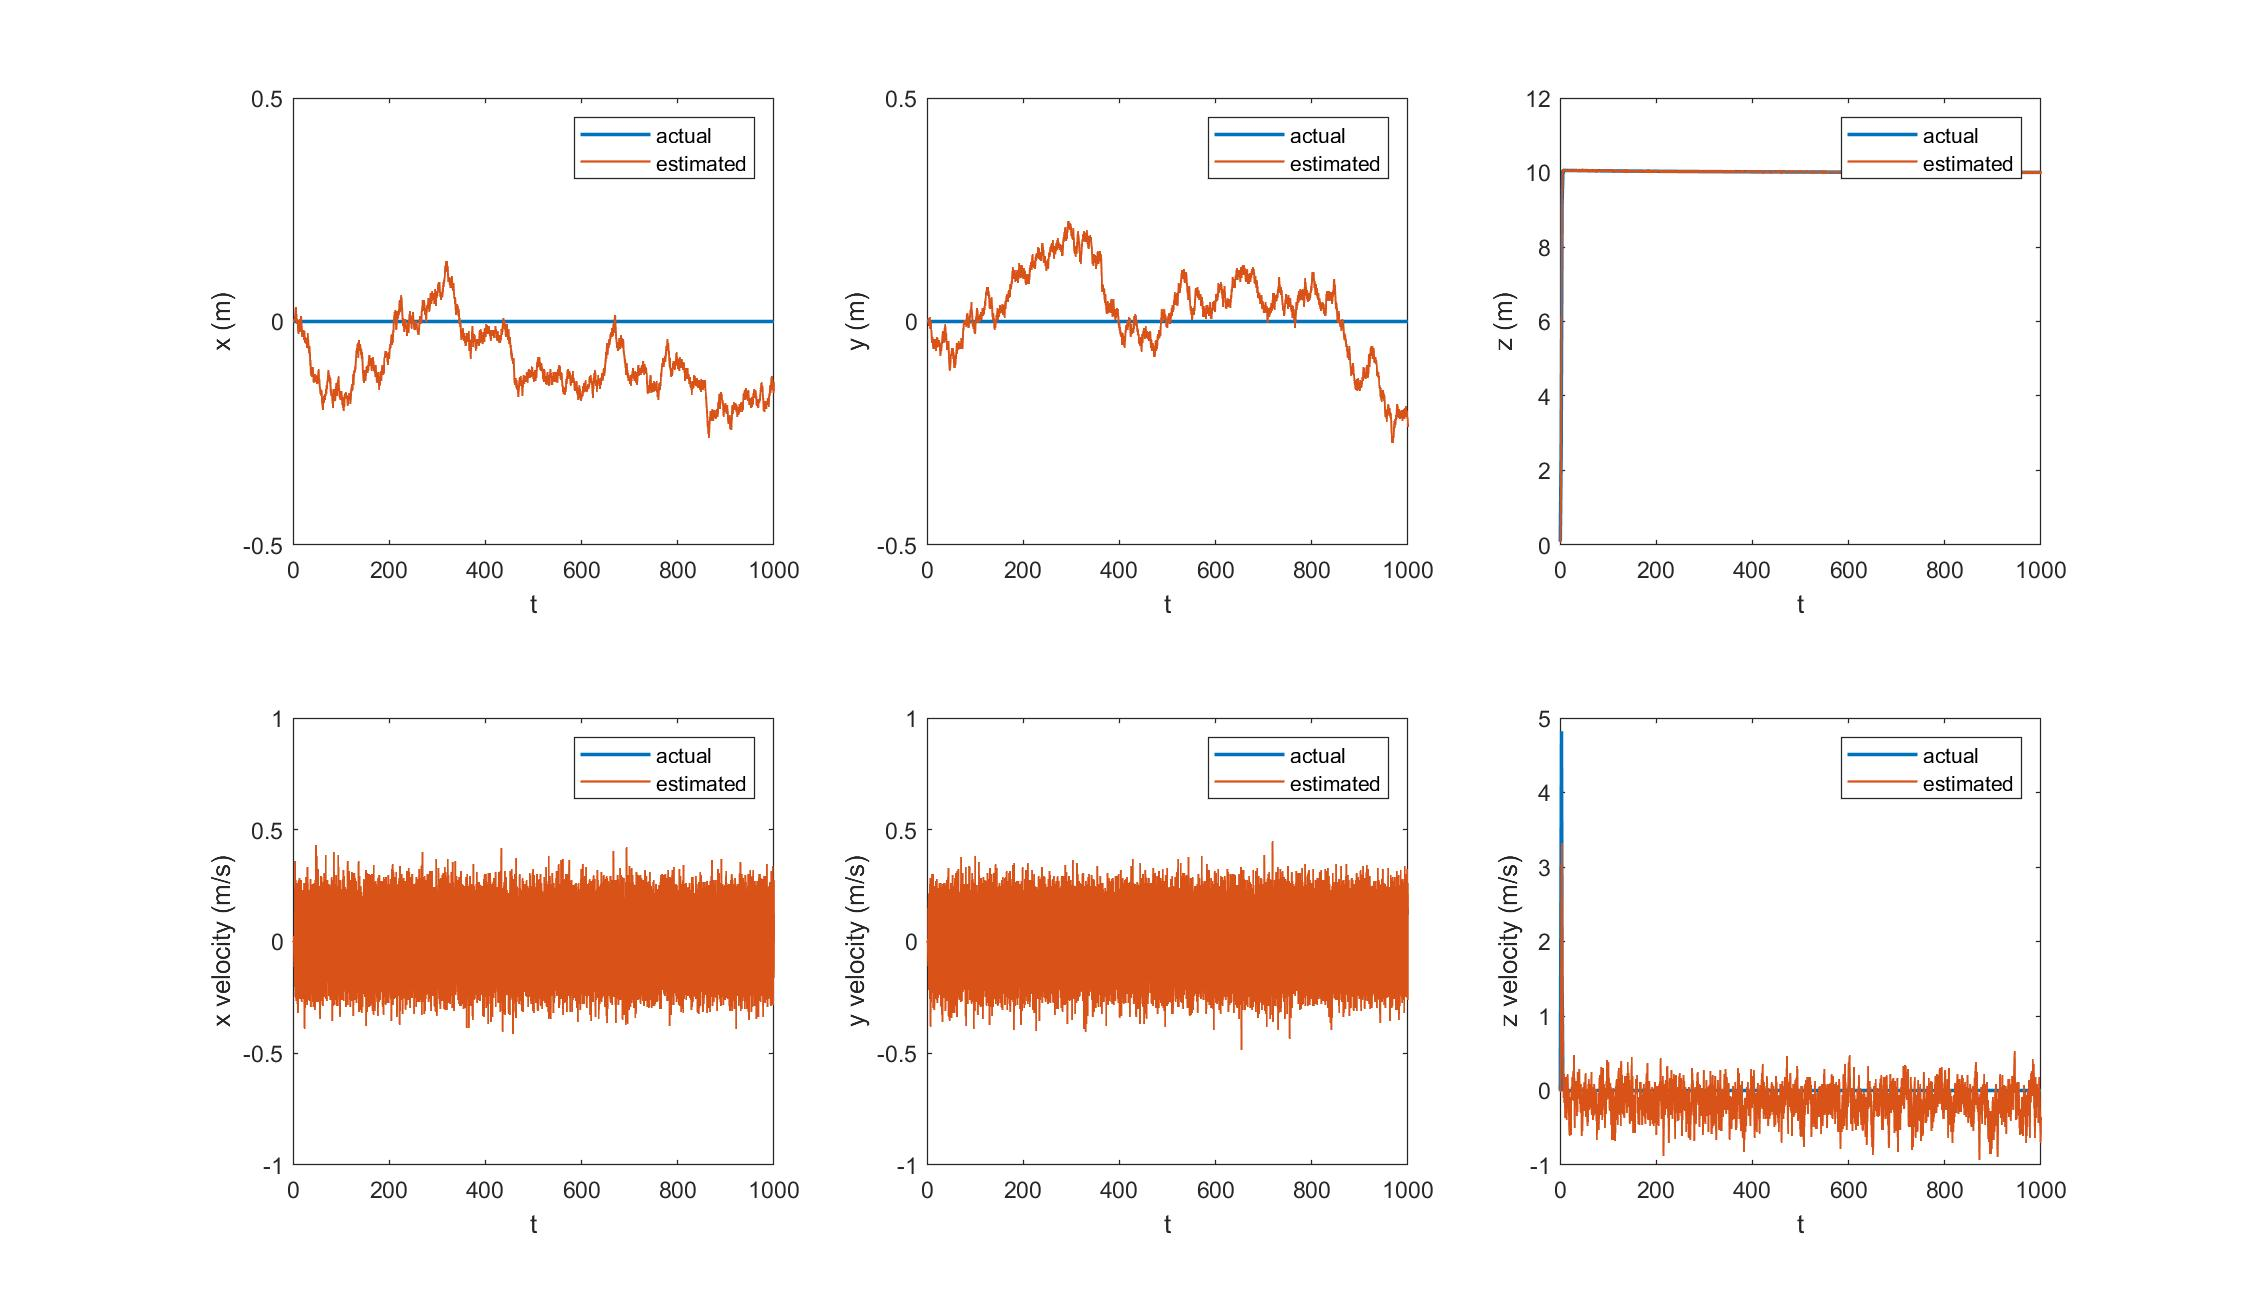
\includegraphics[width=\columnwidth]{/EKF_OFS/Drift.jpg}\\
	\end{center}
	\caption{Estimated translational states over 1000 seconds.}%
	\label{fig:EKF_OFS_Drift}%
\end{figure}

\figref{fig:EKF_OFS_3D} visually compares the vehicle's simulated position with its estimated position in 3D space, whilst moving between a number of waypoints. It can be seen that, although there is no GPS data available a fairly accurate position estimate can be maintained even whilst the vehicle is tracking waypoints.
\begin{figure}[htb]
\begin{center}
	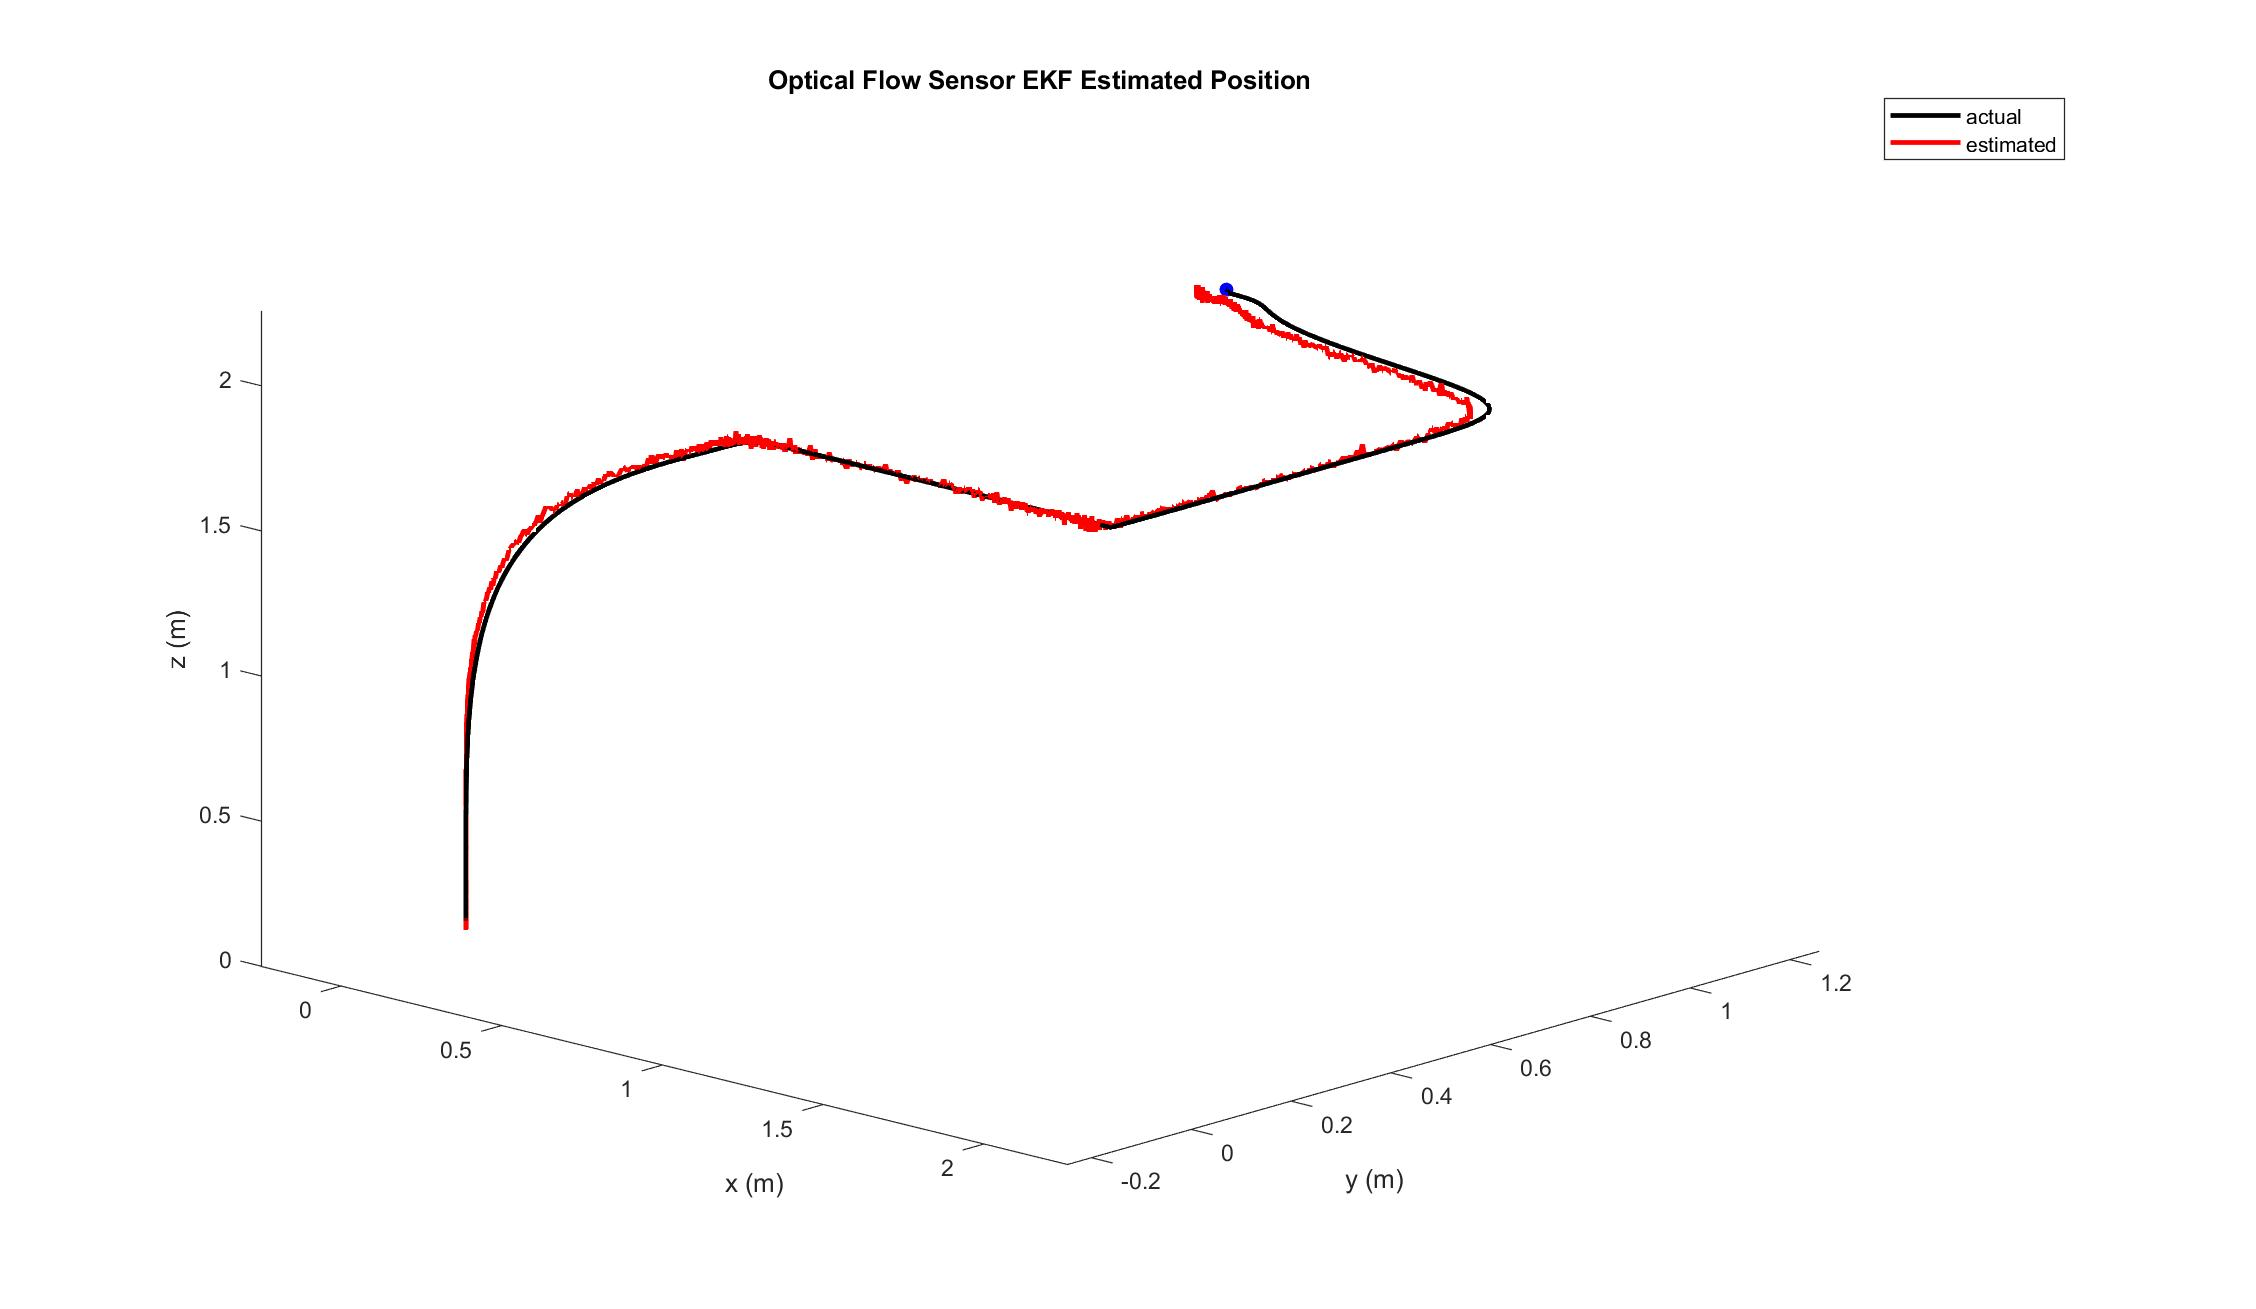
\includegraphics[width=\columnwidth]{/EKF_OFS/Waypoints.jpg}\\
	\end{center}
	\caption{Estimated position of the vehicle in 3D space while moving between waypoints over a period of 20 seconds.}%
	\label{fig:EKF_OFS_3D}%
\end{figure}


A more accurate and reliable EKF would utilise all of the previously mentioned sensors i.e. GPS, barometer, OFS and lidar. 

\FloatBarrier

\section{Chapter Summary}
This chapter developed two sensor fusion algorithms based on the extended Kalman filter. The first algorithm utilises GPS data to estimate position. The second estimator utilises an optical flow sensor and does not rely on GPS. This has the advantage of allowing UAV operation in areas which have limited GPS signal, but is limited to operating with unobstructed line of sight to the ground. A more reliable sensor fusion algorithm would include the use of both groups of sensors.

\clearpage


